%!TEX root = ../main.tex
% file: assignment2.tex


\graphicspath{{C:/Documents and Settings/amcelhinney/My Documents/GitHub/MCS507HW/MCS 507 Homework 4/MCS507--Project-3/tex/include/}}

\section{Assignment One: Overview and Illustrative Example} % (fold)
\label{sec: Main Problem}
Our first objective is to identify the main problem this technique aims to solve. We then provide an overview of the techniques and their implementation. We conclude with an illustrative example that displays the utility of this software.

\subsection{Main Problem this Technique Aims to Solve} % (fold)
\label{sub:methoda}
Bayesian Classifiers broadly refers to a class of tools that rely on Bayes rule to classify objects into various categories. Classification problems are found in nearly every aspect of academic and industrial researching. In particular, Bayesian techniques have proven to be extremely versatile. They have many broad applications in industry and academia. Applications of Bayesian classifiers are found in:

\begin{enumerate}
\item Spam detection
\item Speech Recognition (Merhav)
\item Diagnosis of Dental Pain (Chattopadhyay 2010)
\item Plant Identification
\end{enumerate}

% subsection Main Problem this Software Aims to Solve (end)

\subsection{Overview of the Theory} % (fold)

As stated, Bayesian Classifiers rely on  Bayes theorem, which states for two events \emph{A} and \emph{B}:

\begin{equation}
P(A|B)=\frac{P(B|A)*P(A)}{P(B)}
\end{equation}

\begin{flushleft}We can extend this theorem to any partition of the event space as:
\end{flushleft}

\begin{equation}
P(A_{i}|B)=\frac{P(B|A_{i})*P(A_{i})}{\sum_{j}P(B|A_{j})*P(A_{j})}
\end{equation}

\begin{flushleft}Based on this simple rule, we can address problems of classification by taking a group of observations whose features are known. Then upon finding a suitable probability distribution, we can use Bayes Theorem to calculate the probability that another observation belongs to a certain class, conditional on its features (StatSoft, 2012). 
\end{flushleft}

% subsection Overview of the Theory (end)

\subsection{Illustrative Example} % (fold)

\begin{flushleft}We can illustrate this concept with an example. Suppose that all football teams are either winners or losers. Further, supposed that there are only two football teams on tv that day: the Chicago Bears and the Green Bay Packers. Since the Chicago Bears are such a superior team, they are winners 80\% of the time and therefore losers 20\% of the time. Whereas the Green Bay packers, being inferior in every way, are winners a mere 10\% of the time and therefore losers 90\% of the time. Now suppose upon turning on ESPN to catch the game scores, you hear them refer to a winning team, but cannot make out the name of the team. You would like to know which team they were discussing, but you know that they were either discussing the Chicago Bears or the Green Bay Packers with equal chance. Thus, we can use Bayes Theorem to represent this problem as:
\end{flushleft}

\begin{equation}
P(Bears|Winner)=\frac{P(Winner|Bears)*P(Bears)}{P(Winner)}
\end{equation}

\begin{equation}
P(Winner)=P(Winner|Bears)*P(Bears)+P(Winner|Packers)*P(Packers)
\end{equation}

\begin{flushleft}Using the known values, \begin{math}P(Winner|Bears)=.9\end{math} and \begin{math}P(Bears)=.5\end{math}, we can compute that \begin{math}P(Winner)=.8*.5+.1*.5=.45\end{math}. Finally, this implies
\end{flushleft}
\begin{equation}
P(Bears|Winner)=\frac{.8*.5}{.45}=89\%
\end{equation}
We can thus conclude with nearly 89\% certainty that they were discussing the Chicago Bears and not the Green Bay Packers.


% subsection Illustrative Example (end)

\subsection{Overview of the Methodology} % (fold)

\begin{flushleft}
Now that we have an understanding of Bayes Theorem, we can further discuss the implementation of it for purposes of a Bayesian Classifier. As previously stated, a Bayesian Classifier builds off Bayes theorem to predict membership to a class. If the classifier uses strict assumptions about the independence of the variables, it is referred to as a Niave Bayes Classifier (How to Build a Naive Bayes Classifier, 2012). 
\end{flushleft}
These classifiers are typically implemented using k-fold cross validation. k-fold cross validation is a commonly used machine learning technique where the data is divided into roughly k equal parts (k being specified by the user at the outset). The model is then fit using the observations in k-1 parts. Then the model is then used to score the k-th part. The accuracy of the model is then computed based on its predictive power for this k-th part. This process is repeated k-times, using a different partition each time. The selection of the value k is somewhat arbitrary, but for large data sets, k=10 is generally accepted as a reasonable choice. 

\begin{figure}[H]
    \centering
       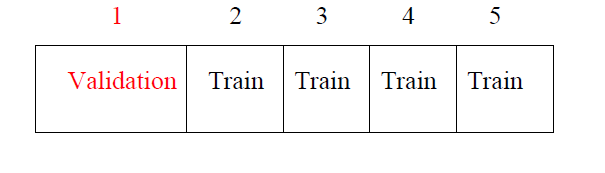
\includegraphics[width=4.5 in]{k-fold_cv.png}
    \caption{Example of k-fold cross-validation, k=5. (Hastie \& Tibshirani 2009)}
    \label{Example Data}
\end{figure}

% subsection Overview of the Methodology (end)

% section Assignment One: Overview and Illustrative Example (end)
